\section{Results from the perpetual youth model}


\subsection{Implied distribution of bank heterogeneity}

\par The simple model of the bank's optimization problem, where the bank cares only about the difference between the market rate  $R^m$  and their chosen level of deposit rate to offer $R^d$  and the level of foreign deposits $S_i(R^d)$, runs into a dilemma for the infinite horizon version of the model. That is, the results of the SMM estimation leave us with 7 discretized points for the uniform distribution of returns $[0.9635, 0.9828, 1.002, 1.0212, 1.0404, 1.0596, 1.0789]$, where the first two points imply a negative return on assets (an issue that does not arise during the estimation of the life-cycle model).

\par Thus, when we inspect the optimal behavior for offered deposit rates and the calibrated value of the market return using the Cobb-douglas production function, we see that the implied elasticities for the first two banks will be negative, which cannot occur. Although it is conceivable for an individual to earn a negative return on their deposits (i.e. the intersection of low offered deposit rates and potentially high banking/overdraft fees), I leave out the computation of the elasticites for this version of the model. Perhaps are more robust description of the bank's optimization problem would allow the infinite horizon setting to not only match the capital-to-output ratio and chosen wealth moements, but also lead to an implied distribution of elasticities with positive support post-estimation. 

\subsection{Untargeted moments}

\par These two tables present the simulated version of the untargeted moments for the infinite horizon version of the  model without heterogeneity~\ref{fig:SimLorenzTarPoint}, and then with heterogeneity~\ref{fig:SimLorenzTarDist}.

\begin{figure}[htbp]
\centering
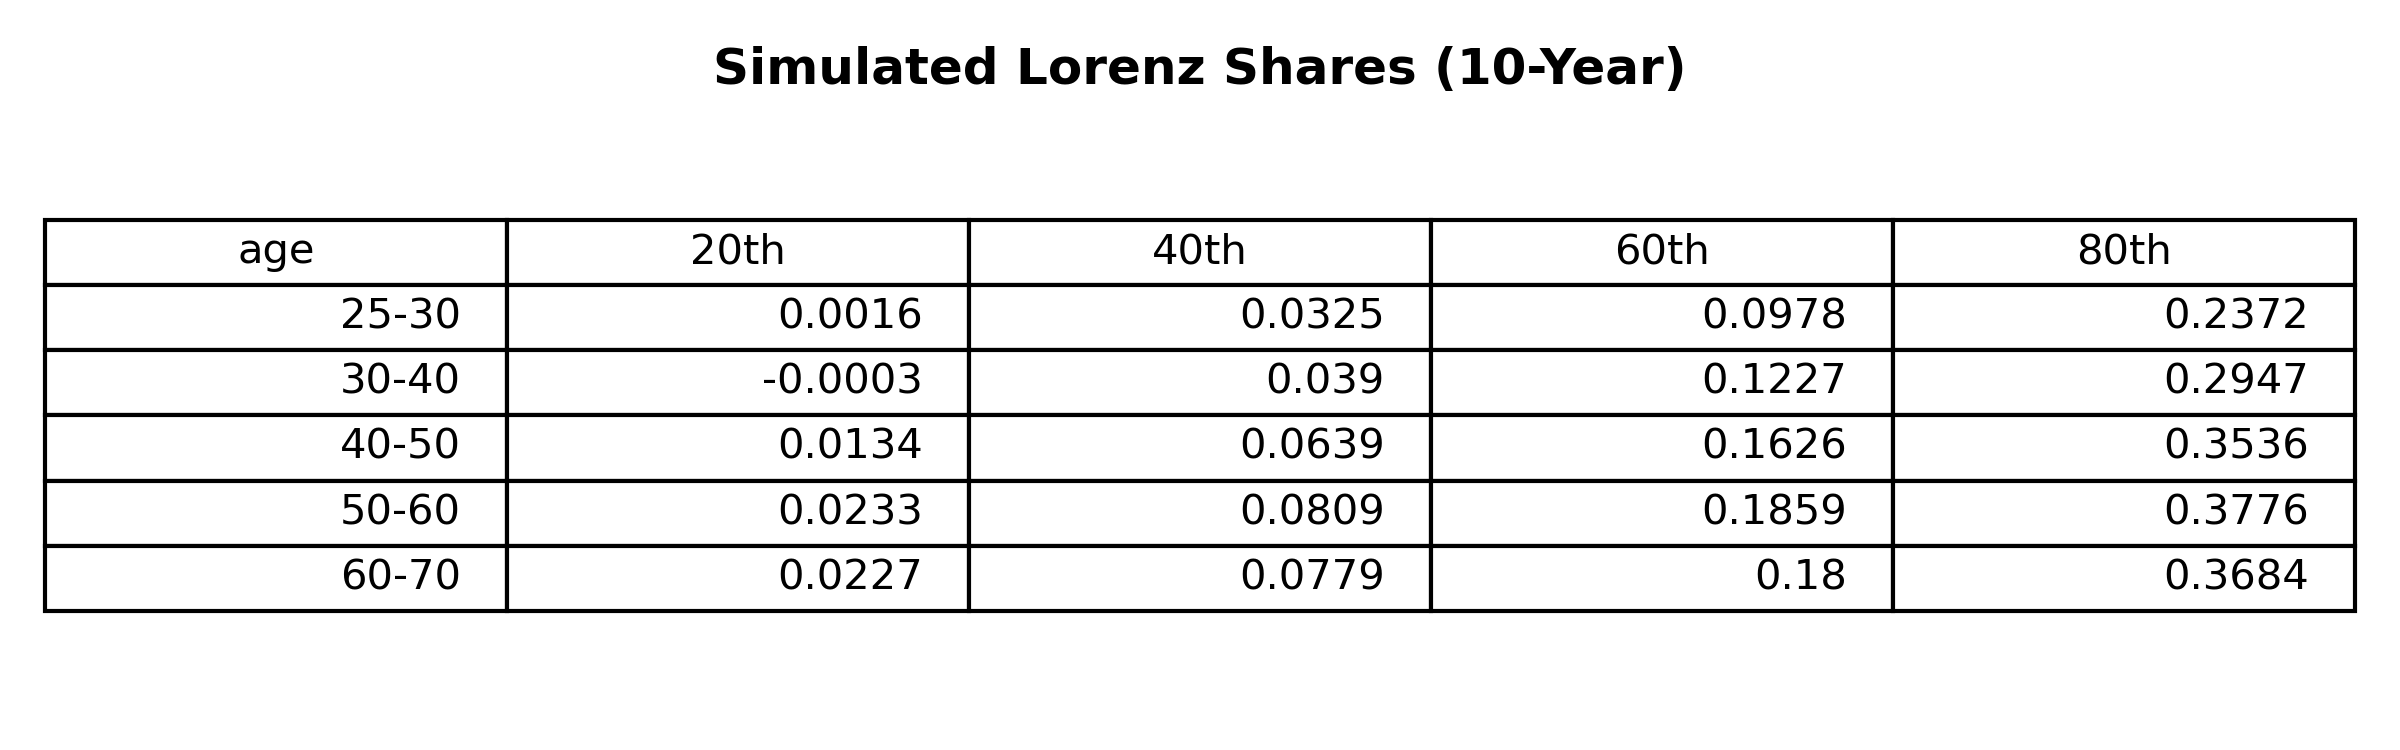
\includegraphics[width=0.8\textwidth]{Tables/Sim_Lorenz_10yr_LCrrPointNetWorth.png}
\caption{Simulated Untargeted Moments without Heterogeneity (R-point).}
\label{fig:SimLorenzTarPoint}
\end{figure}

\begin{figure}[htbp]
\centering
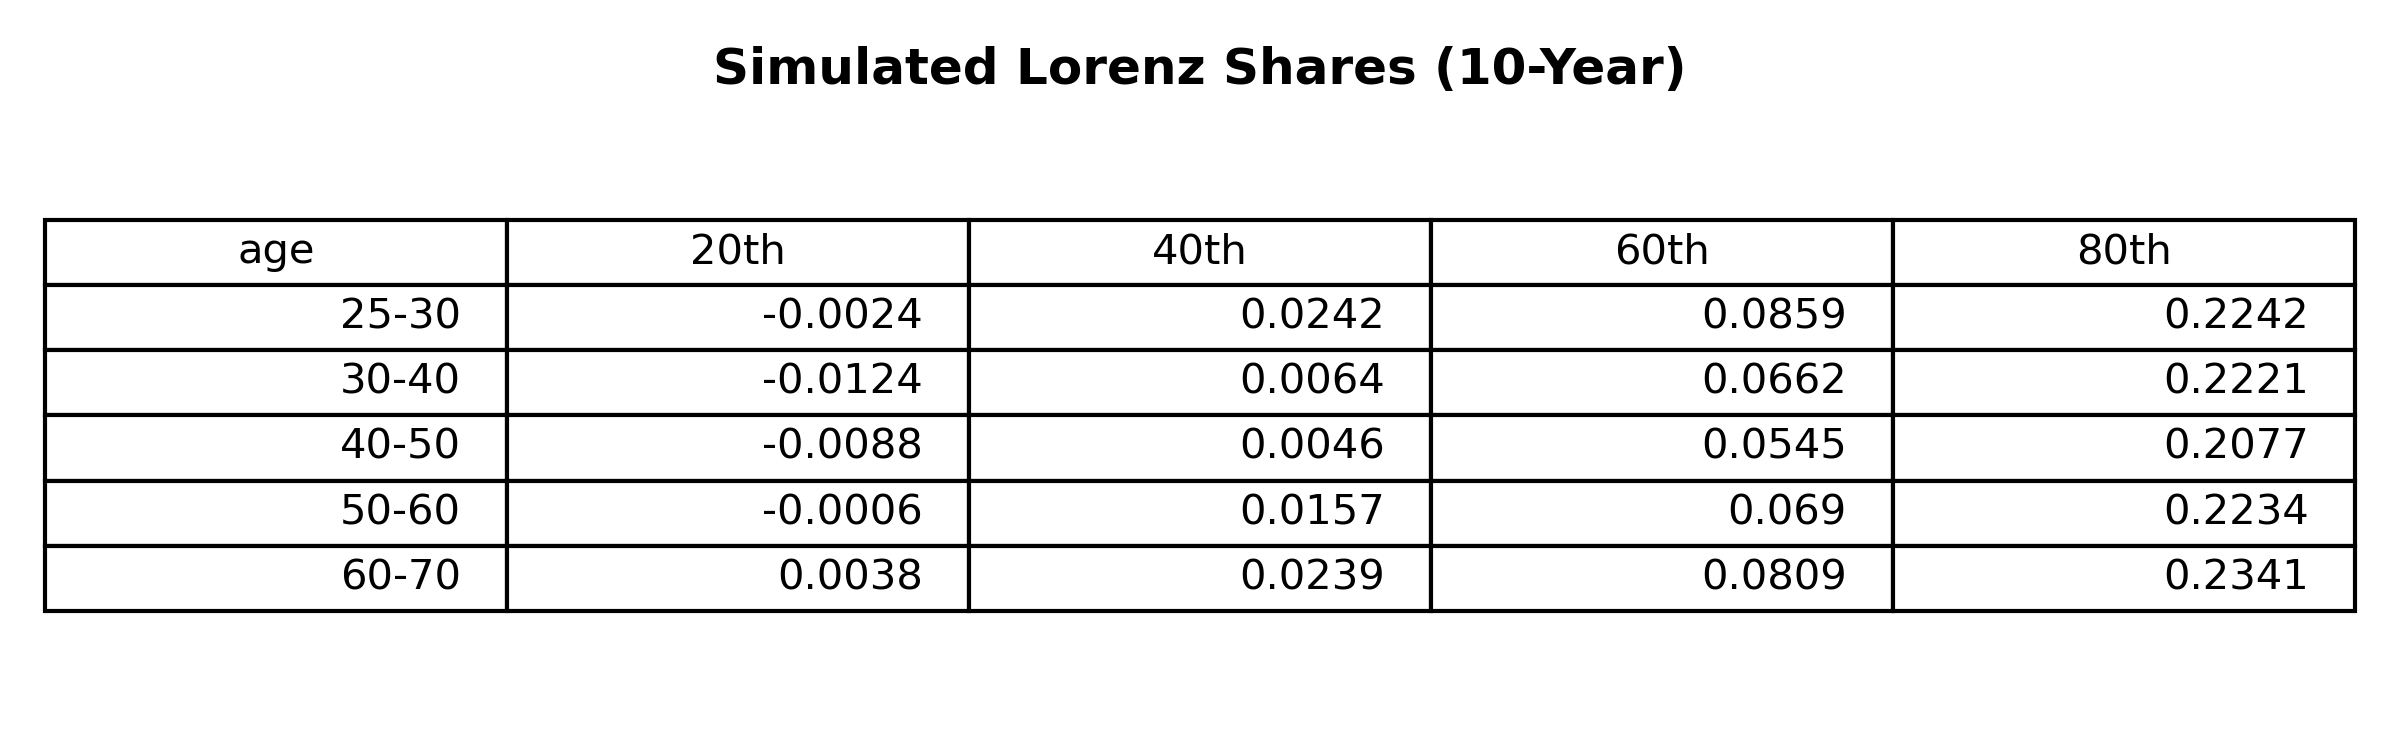
\includegraphics[width=0.8\textwidth]{Tables/Sim_Lorenz_10yr_LCrrDistNetWorth.png}
\caption{Simulated Untargeted Moments with Heterogeneity (R-dist).}
\label{fig:SimLorenzTarDist}
\end{figure}
